\documentclass[14pt,aspectratio=1610]{beamer}

\usepackage[brazil]{babel}
\usepackage[utf8]{inputenc}
%\UseRawInputEncoding
\usepackage[T1]{fontenc}
%\usepackage{Sweave}
\usepackage{animate}
\usepackage{amsbsy}
\usepackage{amsfonts}
\usepackage{amsmath}
\usepackage{amssymb}
\usepackage{amsthm}
\usepackage[toc,page,title,titletoc]{appendix}
%\usepackage[fixlanguage]{babelbib}
%\usepackage[pdftex]{color}
\usepackage{dsfont}
\usepackage{esvect}
\usepackage[labelfont=bf]{caption}
\usepackage{subcaption}
\usepackage{float}
\usepackage[Glenn]{fncychap}%Sonny %Conny %Lenny %Glenn %Renje %Bjarne %Bjornstrup
%\usepackage{geometry, calc, color, setspace}%
%\geometry{a4paper, headsep=1.0cm, footskip=1cm, lmargin=3cm, rmargin=2cm, tmargin=3cm, bmargin=2cm}
\usepackage{graphicx}
\usepackage{indentfirst}%Para indentar os parágrafos automáticamente
\usepackage{lipsum}
\usepackage{longtable}
\usepackage{mathtools}
\usepackage{listings}%Inserir codigo do R no latex
%\usepackage{slashbox}
\usepackage{multirow}
\usepackage{multicol}
\usepackage{natbib}
\setcitestyle{authoryear,open={(},close={)}} %Citation-related commands
\bibliographystyle{abbrvnat}
%\usepackage{csquotes}
%\usepackage[natbib=true,style=abnt, sorting=none]{biblatex}
%\addbibresource{bibliografia.bib}
\usepackage[figuresright]{rotating}
\usepackage{spalign}
%\usepackage{pgfpages}
\usepackage{pgfplots}
\pgfplotsset{compat=1.18}
\usepackage{tikz}
\usepackage{color, colortbl}
\usepackage{ragged2e}%para justificar o texto dentro de algum ambiente
\definecolor{Gray}{gray}{0.9}
\definecolor{LightCyan}{rgb}{0.88,1,1}
\definecolor{Lightblue}{RGB}{50, 149, 168}
%\usepackage{grffile}

\usepackage[all]{xy}



\usetheme{Madrid}
\usecolortheme[RGB={193,0,0}]{structure}

%\setbeamertemplate{footline}[frame number]
%\setbeamertemplate{footline}[text line]{%
%  \parbox{\linewidth}{\vspace*{-8pt}\hfill\date{}\hfill\insertshortauthor\hfill\insertpagenumber}}
\beamertemplatenavigationsymbolsempty
\renewcommand{\vec}[1]{\mbox{\boldmath$#1$}}
\newtheorem{Teorema}{Teorema}
\newtheorem{Proposicao}{Proposição}
\newtheorem{Definicao}{Definição}
\newtheorem{Corolario}{Corolário}
\newtheorem{Demonstracao}{Demonstração}
\newcommand{\bx}{\ensuremath{\bar{x}}}
\newcommand{\Ho}{\ensuremath{H_{0}}}
\newcommand{\Hi}{\ensuremath{H_{1}}}
\everymath{\displaystyle}

\apptocmd{\frame}{}{\justifying}{} % Allow optional arguments after frame.

\title{Iniciação à Estatística}
\author{Prof. Fernando de Souza Bastos \texorpdfstring{\\ fernando.bastos@ufv.br}{}}
\institute{Departamento de Estatística \texorpdfstring{\\ Universidade Federal de Viçosa}{}\texorpdfstring{\\ Campus UFV - Viçosa}{}}
\date{}
\newcommand\mytext{Aula 4}
\newcommand\mytextt{Fernando de Souza Bastos}
\newcommand\mytexttt{\url{https://ufvest.github.io/}}

\makeatletter
\setbeamertemplate{footline}
{
  \leavevmode%
  \hbox{%
  \begin{beamercolorbox}[wd=.3\paperwidth,ht=2.25ex,dp=1ex,center]{author in head/foot}%
    \usebeamerfont{author in head/foot}\mytext
  \end{beamercolorbox}%
  \begin{beamercolorbox}[wd=.3\paperwidth,ht=2.25ex,dp=1ex,center]{title in head/foot}%
    \usebeamerfont{title in head/foot}\mytextt
  \end{beamercolorbox}%
  \begin{beamercolorbox}[wd=.35\paperwidth,ht=2.25ex,dp=1ex,right]{site in head/foot}%
    \usebeamerfont{site in head/foot}\mytexttt\hspace*{2em}
    \insertframenumber{} / \inserttotalframenumber\hspace*{2ex} 
  \end{beamercolorbox}}%
  \vskip0pt%
}
\makeatother

\providecommand{\arcsin}{} \renewcommand{\arcsin}{\hspace{2pt}\textrm{arcsen}}
\providecommand{\sin}{} \renewcommand{\sin}{\hspace{2pt}\textrm{sen}}
%\newtheorem{Teorema}{Teorema}
%\newtheorem{Proposicao}{Proposição}
%\newtheorem{Definicao}{Definição}
%\newtheorem{Corolario}{Corolário}
%\newtheorem{Demonstracao}{Demonstração}

\titlegraphic{\hspace*{8cm}\href{https://fsbmat-ufv.github.io/}{
\includegraphics[width=2cm]{Aula4Regressao/Figuras/mylogo.png}}
}


\usepackage{hyperref,bookmark}
\hypersetup{
  colorlinks=true,
  linkcolor=blue,
  citecolor=red,
  filecolor=blue,
  urlcolor=blue,
}

% Layout da pagina
\hypersetup{pdfpagelayout=SinglePage}
\begin{document}
%\input{Aula17-concordance}

\frame{\titlepage}

\begin{frame}{}
\frametitle{\bf Sumário}
\tableofcontents
\end{frame}
\section{Regressão Linear Simples}
\begin{frame}{}
\frametitle{ }
\begin{block}{}
\justifying
Em certas situações podemos estar interessados em descrever a relação entre duas variáveis, e também predizer o valor de uma a partir de outra. Por exemplo, se sabemos a altura de um certo estudante, mas não o seu peso, qual seria um bom chute para o peso deste estudante? 
\end{block}
\end{frame}

\begin{frame}[fragile]{}
\frametitle{ }
\begin{block}{}
\begin{center}
%\begin{Schunk}
%\begin{Sinput}

\begin{verbatim}
x = c(176, 154, 138, 196, 132, 176, 181, 169, 150, 175)
y = c(82, 49, 53, 112, 47, 69, 77, 71, 62, 78)
plot(x,y,xlab="Altura (cm)",ylab="Peso (kg)",
      pch=16, ylim = c(40,115))
lines(x, fitted(lm(y ~ x)), col="blue")    
\end{verbatim}

%\end{Sinput}
%\end{Schunk}
\end{center}
\end{block}
\vspace{-1.3cm}
\begin{center}
\setkeys{Gin}{width=0.5\linewidth}
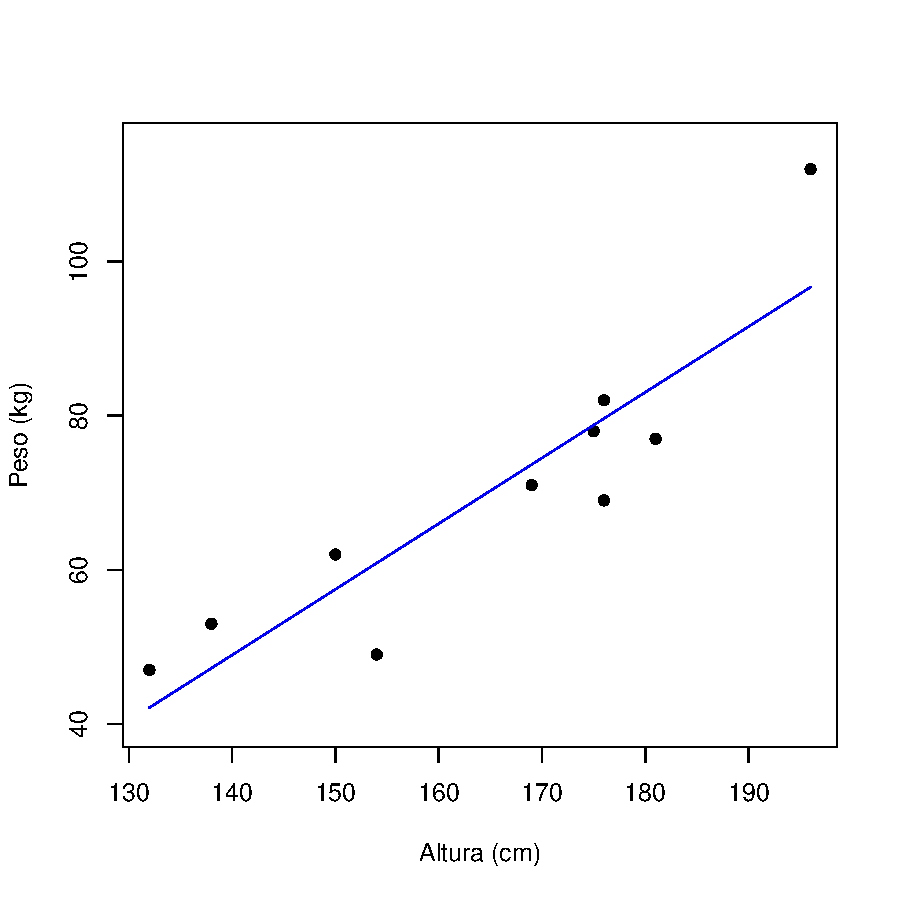
\includegraphics{Aula4Regressao/Figuras/Aula4-002.pdf}
\end{center}
\end{frame}

\begin{frame}[fragile]{}
\frametitle{ }
\begin{block}{}
\begin{center}
%\begin{Schunk}
%\begin{Sinput}
\begin{verbatim}
doses <- c(0, 50, 100, 150, 200, 250, 300)
resp <- c(148.6, 153.6, 154.5, 154.9, 158, 160, 154.4)
reglin <- lm(resp ~ doses) 
plot(doses, resp) #(variável indep. primeiro)
lines(doses, fitted(reglin), col="blue")#acrescenta 
a reta de regressão ajustada
\end{verbatim}
%\end{Sinput}
%\end{Schunk}
\end{center}
\end{block}
\vspace{-1.3cm}
\begin{center}
\setkeys{Gin}{width=0.5\linewidth}
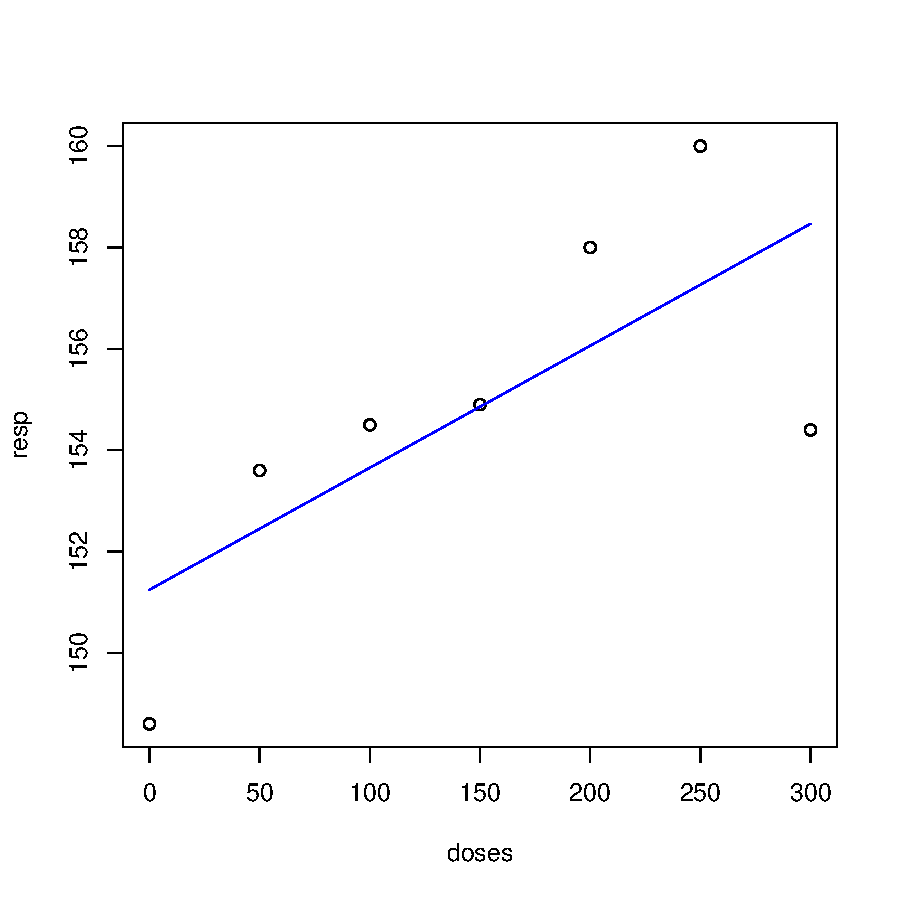
\includegraphics{Aula4Regressao/Figuras/Aula4-004.pdf}
\end{center}
\end{frame}

\begin{frame}[fragile]{}
\frametitle{ }
\begin{block}{}
\begin{center}
%\begin{Schunk}
%\begin{Sinput}
\begin{verbatim}
#Tempo de espera entre erupções e a duração da erupção
fit <- lm(waiting~eruptions, data=faithful)
plot(faithful)
lines(faithful$eruptions, fitted(fit), col="blue")
\end{verbatim}
%\end{Sinput}
%\end{Schunk}
\end{center}
\end{block}
\vspace{-1.3cm}
\begin{center}
\setkeys{Gin}{width=0.5\linewidth}
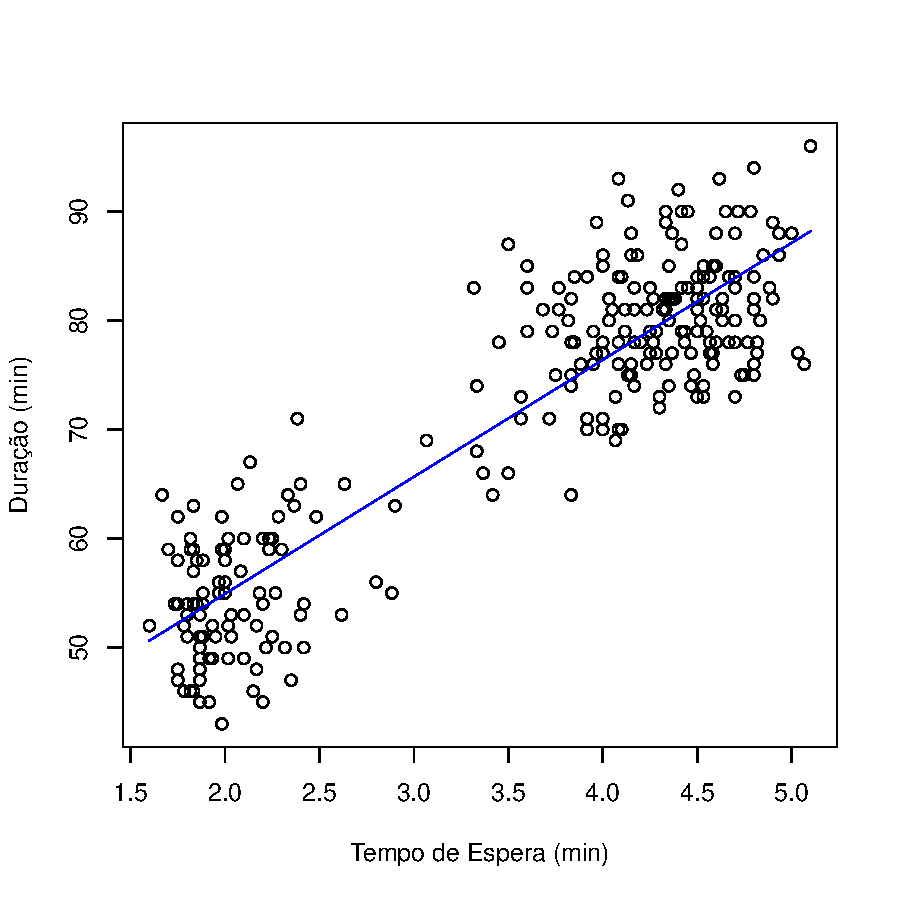
\includegraphics{Aula4Regressao/Figuras/Aula4-006}
\end{center}
\end{frame}

\begin{frame}{}
\frametitle{Objetivos:}
\begin{block}{}
\justifying
Estudar a relação linear entre duas variáveis quantitativas. Exemplos:
\begin{enumerate}[(i)]
\item Altura dos pais e altura dos filhos;\pause
\item Renda semanal e despensas de consumo;\pause
\item Variação dos salários e taxa de desemprego;\pause
\item Demanda dos produtos de uma firma e publicidade;\pause
\end{enumerate}
\end{block}
\begin{block}{}
\justifying
Sob dois pontos de vista:
\begin{enumerate}[(i)]
\item Explicitando a forma dessa relação: regressão.\pause
\item Quantificando a força dessa relação: correlação.
\end{enumerate}
\end{block}
\end{frame}

\begin{frame}{}
\frametitle{ }
\begin{block}{Importante:}
\justifying
Uma relação estatística por sí propria não implica uma causa, para atribuir causa, devemos invocar alguma teoría!
\end{block}
\pause
\begin{block}{}
\justifying
Uma regressão espúria é uma relação estatística existente entre duas variáveis, mas onde não existe nenhuma relação causa-efeito entre elas. Essa relação estatística pode ocorrer por pura coincidência ou por causa de uma terceira variável. Ou seja, neste último caso, pode ocorrer que as variáveis X e Y sejam correlacionadas porque ambas são causadas por uma terceira variável Z.
\end{block}
\end{frame}

\begin{frame}{}
\frametitle{ }
\begin{block}{}
\justifying
Só porque (A) acontece juntamente com (B) não significa que (A) causa (B). Determinar se existe de fato uma relação de causalidade requer  investigação adicional pois podem acontecer cinco situações:
\begin{enumerate}[(i)]
\item (A) causa realmente (B);\pause
\item (B) pode ser a causa de (A);\pause
\item Um terceiro factor (C) pode ser causa tanto de (A) como de (B);\pause
Pode ser uma combinação das três situações anteriores. Por exemplo, (A) causa (B) e ao mesmo tempo (B) causa também (A);\pause
\item A correlação pode ser apenas uma coincidência, ou seja, os dois eventos não têm qualquer relação para além do fato de ocorrerem ao mesmo tempo. 
\end{enumerate}
\end{block}
\end{frame}

\begin{frame}{}
\frametitle{Exemplos:}
\begin{block}{}
\justifying
``Quanto maiores são os pés de uma criança, maior a capacidade para resolver problemas de matemática. Portanto, ter pés grandes faz ter melhores notas em matemática". 
\end{block}
\end{frame}

\begin{frame}{}
\frametitle{Exemplos:}
\begin{block}{}
\justifying
``Vários estudos apontavam inicialmente que as mulheres em menopausa que recebiam terapia de substituição hormonal (TSH) tinham também um menor risco de doença coronária, o que levou à ideia de que a TSH conferia protecção contra a doença coronária. No entanto, estudos controlados e randomizados (mais rigorosos), feitos posteriormente, mostraram que a TSH causava na verdade um pequeno mas significativo aumento do risco de doença coronária. Uma reanálise dos estudos revelou que as mulheres que recebiam a TSH tinham também uma maior probabilidade de pertencer a uma classe socioeconómica superior, com melhor dieta e hábitos de exercício. A utilização da TSH e a baixa incidência de doença coronária não eram causa e efeito, mas o fruto de uma causa comum". 
\end{block}
\end{frame}

\begin{frame}{}
\frametitle{ }
\begin{block}{}
\justifying
``Quanto menos as pessoas se divorciam em Maine (EUA), menor fica o consumo de margarina naquele Estado". 
\end{block}
\begin{figure}[H]
    \centering
    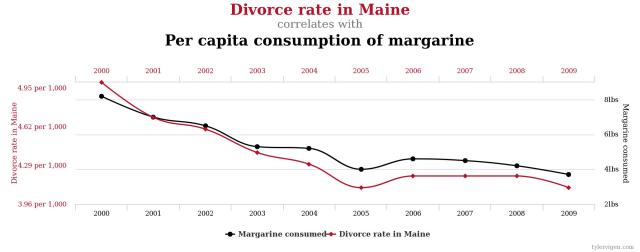
\includegraphics[scale=0.5]{Figuras/Margarina}
    %\caption{Legenda}
    %\label{figRotulo}
\end{figure}
\end{frame}

\begin{frame}{}
\frametitle{ }
\begin{block}{}
\justifying
Deveríamos banir Nicolas Cage do cinema para evitar o afogamento de pessoas? O primeiro gráfico nos dá o número de pessoas afogadas (linha vermelha) e as aparições do Nicolas Cage em filmes (linha preta).
\end{block} 
\begin{figure}[H]
    \centering
    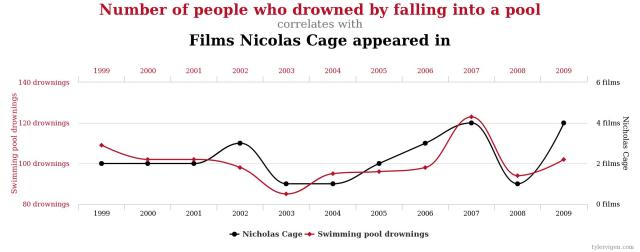
\includegraphics[scale=0.5]{Figuras/Nicolas}
    %\caption{Legenda}
    %\label{figRotulo}
\end{figure}
\end{frame}

\begin{frame}{}
\frametitle{ }
\begin{block}{}
\justifying
Consumo de muçarela (linha vermelha) e doutorados obtidos em engenharia civil (linha preta)
%http://www.tylervigen.com/spurious-correlations
\end{block}
\begin{figure}[H]
    \centering
    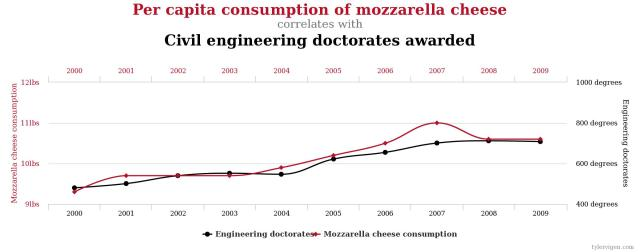
\includegraphics[scale=0.5]{Figuras/Mucarela}
    %\caption{Legenda}
    %\label{figRotulo}
\end{figure}
\end{frame}

\begin{frame}{}
\frametitle{ }
\begin{block}{}
\justifying
De forma geral, um modelo estatístico pode ser escrito da seguinte forma:

$$Y=\textrm{componente determinística}+\textrm{componente aleatória}$$

existem diversas maneiras de específicar essas componentes. Começaremos com uma regressão linear simples.

\end{block}
\end{frame}


\begin{frame}{}
\frametitle{ }
\begin{block}{}
\justifying
Uma regresão linear simples tem como objetivo aproximar uma variável resposta $Y$ através de uma função linear de uma variável de interesse, ou seja,

$$Y=f(X,\beta)+\varepsilon=\beta_{0}+\beta_{1}X+\varepsilon$$

No qual assume-se que:

\begin{enumerate}[(i)]
\item $E(\varepsilon)=0$\pause
\item $V(\varepsilon)=\sigma^{2}$ (Homocedásticidade)\pause
\item $Cov(\varepsilon_{i},\varepsilon_{j})=0$
\end{enumerate}

em outras palavras, os erros tem média zero, variância constante e são não correlacionados.

\end{block}
\end{frame}

\begin{frame}{}
\frametitle{ }
\begin{block}{}
\justifying
A variável preditora $X$ pode vir de diversas fontes:
\begin{itemize}
\item inputs quantitativos (valores reais, medidas)
\item tranformação de variável quantitativas ($\log()$ ,$\sqrt()$,etc)
\item inputs qualitativos (``dummy" e.x. genêro, classes)
\end{itemize}
Dessa forma, um modelos de regressão consiste em 4 passos:
\begin{enumerate}
\item Escolher o componente determinístico do modelo;\pause
\item Especificar a distribuição do erro;\pause
\item Utilizar os dados para estimar os parâmetros do modelo;\pause
\item Avaliar o modelo estatístico;
\end{enumerate}
\end{block}
\end{frame}


\begin{frame}{}
\frametitle{ }
\begin{block}{}
\justifying
Os dados para a análise de regressão e correlação simples são da forma:
$$(x_{1},y_{1}),(x_{2},y_{2}),\cdots, (x_{n},y_{n})$$

Com base nos dados constrói-se o diagrama de dispersão, que deve exibir
uma tendência linear para que se possa usar a regressão linear.
Este diagrama permite decidir empiricamente:
\begin{itemize}
\item Se um relacionamento linear entre as variáveis $X$ e $Y$ deve ser assumido;
\item Se o grau de relacionamento linear entre as variáveis é forte ou fraco,
conforme o modo como se situam os pontos em redor de uma reta imaginária que passa através do enxame de pontos.
\end{itemize}
\end{block}
\end{frame}

\begin{frame}[fragile]{}
\frametitle{ }
\begin{block}{}
\begin{center}
%\begin{Schunk}
%\begin{Sinput}
\begin{verbatim}
#Encontre o modelo de Regressão Linear que melhor se
ajusta aos dados
x = c(176, 154, 138, 196, 132, 176, 181, 169, 150, 175)
y = c(82, 49, 53, 112, 47, 69, 77, 71, 62, 78)    
\end{verbatim}
%\end{Sinput}
%\end{Schunk}
\end{center}
\end{block}
\vspace{-1.3cm}
\begin{center}
\setkeys{Gin}{width=0.5\linewidth}
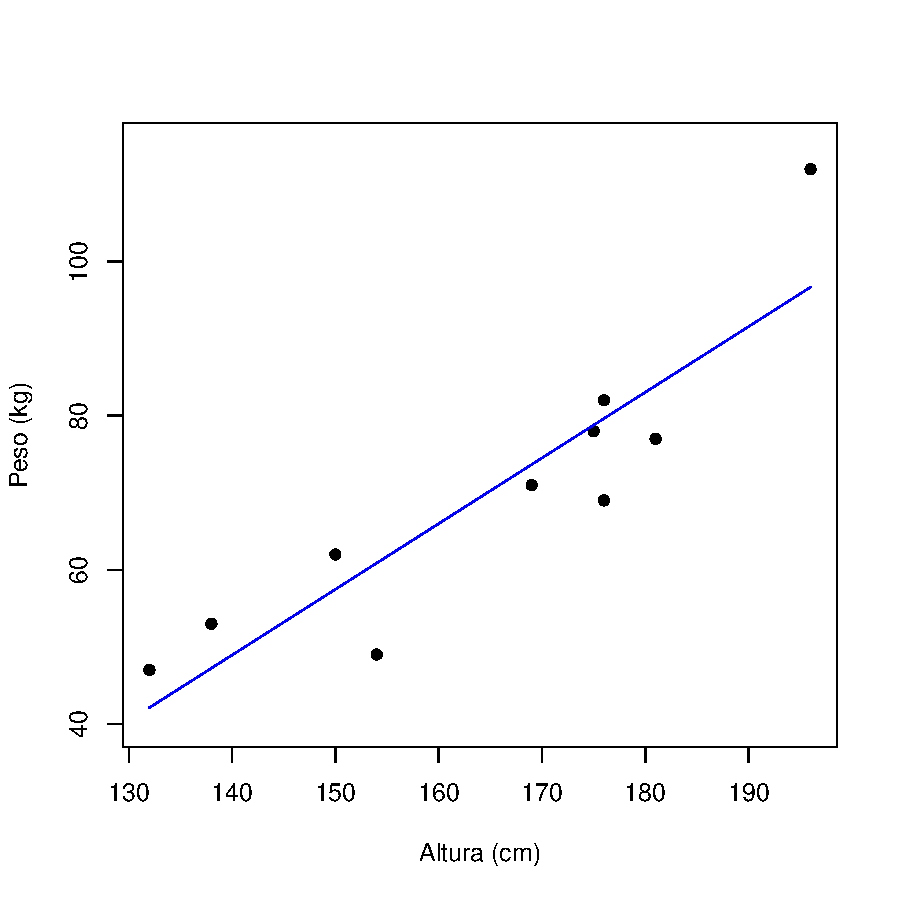
\includegraphics{Aula4Regressao/Figuras/Aula4-008}
\end{center}
\end{frame}

\begin{frame}[fragile]{}
\frametitle{ }
\begin{block}{}
\begin{center}
%\begin{Schunk}
%\begin{Sinput}
\begin{verbatim}
#Encontre o modelo de Regressão Linear que melhor se
ajusta aos dados
x <-  c(176, 154, 138, 196, 132, 176, 181, 169, 150, 175)
y <-  c( 82,  49,  53, 112,  47,  69,  77,  71,  62,  78)
Reg <- lm(y~x)
Reg    
\end{verbatim}
%\end{Sinput}
%\begin{Soutput}
\begin{verbatim}
Call:
lm(formula = y ~ x)

Coefficients:
(Intercept)            x  
   -70.4627       0.8528     
\end{verbatim} 
%\end{Soutput}
%\end{Schunk}
\end{center}
\end{block}
\end{frame}

\begin{frame}[fragile]{}
\frametitle{ }
\begin{block}{}
\begin{center}
%\begin{Schunk}
%\begin{Sinput}
\begin{verbatim}
#library(texreg)
summary(Reg)    
\end{verbatim}
%\end{Sinput}
%\begin{Soutput}
\begin{verbatim}
lm(formula = y ~ x)
Residuals:
     Min       1Q   Median       3Q      Max 
-11.8746  -5.8428   0.7893   4.8001  15.3061 
Coefficients:
            Estimate Std. Error t value Pr(>|t|)    
(Intercept) -70.4627    24.0148  -2.934 0.018878 *  
x             0.8528     0.1448   5.889 0.000366 ***
Signif. codes:  0 '***' 0.001 '**' 0.01 '*' 0.05 '.' 
Residual standard error: 8.854 on 8 degrees of freedom
Multiple R-squared:  0.8126,	Adjusted R-squared:  0.7891 
F-statistic: 34.68 on 1 and 8 DF,  p-value: 0.0003662  
\end{verbatim}
%\end{Soutput}
%\end{Schunk}
\end{center}
\end{block}
\end{frame}

% \begin{frame}{}
% \frametitle{ }
% \begin{block}{}
% \justifying
% \begin{table}[H] 
% \centering 
% \caption{} 
% \label{} 
% \begin{tabular}{@{\extracolsep{5pt}}lc} 
% \\[-1.8ex]\hline 
% \hline \\[-1.8ex] 
%  & \multicolumn{1}{c}{\textit{Dependent variable:}} \\ 
% \cline{2-2} 
% \\[-1.8ex] & y \\ 
% \hline \\[-1.8ex] 
%  x & 0.853$^{***}$ \\ 
%   & (0.145) \\ 
%   & \\ 
%  Constant & $-$70.463$^{**}$ \\ 
%   & (24.015) \\ 
%   & \\ 
% \hline \\[-1.8ex] 
% Observations & 10 \\ 
% R$^{2}$ & 0.813 \\ 
% Adjusted R$^{2}$ & 0.789 \\ 
% Residual Std. Error & 8.854 (df = 8) \\ 
% F Statistic & 34.682$^{***}$ (df = 1; 8) \\ 
% \hline 
% \hline \\[-1.8ex] 
% \textit{Note:}  & \multicolumn{1}{r}{$^{*}$p$<$0.1; $^{**}$p$<$0.05; $^{***}$p$<$0.01} \\ 
% \end{tabular} 
% \end{table} 
% \end{block}
% \end{frame}

\begin{frame}{}
\frametitle{ }
\begin{block}{}
\begin{table}
\begin{center}
\begin{tabular}{lc}
\hline
 & Model 1 \\
\hline
(Intercept) & $-70.46^{*}$ \\
            & $(24.01)$    \\
x           & $0.85^{***}$ \\
            & $(0.14)$     \\
\hline
R$^2$       & 0.81         \\
Adj. R$^2$  & 0.79         \\
Num. obs.   & 10           \\
RMSE        & 8.85         \\
\hline
\multicolumn{2}{l}{\scriptsize{$^{***}p<0.001$, $^{**}p<0.01$, $^*p<0.05$}}
\end{tabular}
\caption{Statistical models}
\label{table:coefficients}
\end{center}
\end{table} 
\end{block}
\end{frame}

\begin{frame}{}
\frametitle{ }
\begin{block}{Raiz Quadrada do Erro Quadrático Médio}
\justifying
ROOT MEAN SQUARE ERROR (RMSE)

A medida de erro mais comumente usada para aferir a qualidade do ajuste de um modelo é a chamada RAIZ DO ERRO MÉDIO QUADRÁTICO. Ela é a raiz do erro médio quadrático da diferença entre a predição e o valor real. Podemos pensar nela como sendo uma medida análoga ao desvio padrão.
 
\end{block}
\end{frame}

\begin{frame}{}
\frametitle{ }
\begin{block}{$R^2$}
\justifying
Representa a porcentagem de variação na resposta que é explicada pelo modelo. Ele é calculado como 1 menos a razão da soma dos quadrados dos erros (que é a variação que não é explicada pelo modelo) pela soma total dos quadrados (que é a variação total no modelo). 

Use $R^{2}$ para determinar se o modelo ajusta bem os dados. Quanto mais alto o valor de $R^{2}$ melhor o modelo ajusta seus dados. O valor de $R^{2}$ está sempre entre 0 e 100%.
\end{block}\pause
\begin{block}{$R^2$}
\justifying
Use $R^{2}$ para determinar se o modelo se ajusta bem aos dados. Quanto mais alto o valor de $R^{2}$ melhor o modelo ajusta seus dados. O valor de $R^{2}$ está sempre entre 0 e $100\%.$
\end{block}
\end{frame}


\begin{frame}{}
\frametitle{Considere as seguintes questões ao interpretar o valor de $R^{2}:$}
\begin{block}{}
\justifying
O $R^{2}$ sempre aumenta quando você adiciona mais preditores a um modelo. Por exemplo, o melhor modelo de cinco preditores terá sempre um $R^{2}$ que é pelo menos tão elevado quanto o melhor modelo de quatro preditores. Portanto, $R^{2}$ é mais útil quando for comparado a modelos do mesmo tamanho. 
\end{block}\pause
\begin{block}{}
\justifying
Amostras pequenas não fornecem uma estimativa precisa da força da relação entre a resposta e os preditores. Se você precisar que $R^{2}$ seja mais exato, deve usar uma amostra maior (geralmente, 40 ou mais). 
\end{block}
\end{frame}

\begin{frame}{}
\frametitle{ }
\begin{block}{}
\justifying
$R^{2}$ é apenas uma medida de o quão bem o modelo ajusta os dados. Mesmo quando um modelo tem um $R^{2}$ elevado, você deve verificar os gráficos de resíduos para conferir se o modelo satisfaz os pressupostos do modelo. 
\end{block}
\end{frame}

\begin{frame}{}
\frametitle{$R^{2}$ Ajustado}
\begin{block}{}
\justifying
O $R^{2}$ ajustado é a porcentagem de variação na resposta que é explicada pelo modelo, ajustada para o número de preditores do modelo em relação ao número de observações. 
\end{block}\pause
\begin{block}{Interpretação:}
\justifying
Use o $R^{2}$ ajustado quando desejar comparar modelos que têm diferentes números de preditores. $R^{2}$ sempre aumenta quando você adiciona um preditor ao modelo, mesmo quando não existe uma verdadeira melhoria ao modelo. O valor de $R^{2}$ ajustado incorpora o número de preditores no modelo para ajudá-lo a escolher o modelo correto. 
\end{block}
\end{frame}

\begin{frame}{}
\frametitle{ }
\begin{block}{}
\justifying
O parâmetro $\beta_0$ é chamado intercepto ou coeficiente linear e representa o ponto em que a reta regressora corta o eixo dos $y's,$ quando $x=0.$ Já o parâmetro $\beta_1$ representa a inclinação da reta regressora e é dito coeficiente de regressão ou coeficiente angular. Além disso, temos que para um aumento de uma unidade na variável $x,$ o valor $E(Y|x)$ aumenta $\beta_1$ unidades. A interpretação geométrica dos parâmetros $\beta_0$ e $\beta_1$ pode ser vista na próxima Figura.
\end{block}
\end{frame}

\begin{frame}{}
\frametitle{ }
\begin{block}{}
\begin{figure}[H]
    \centering
    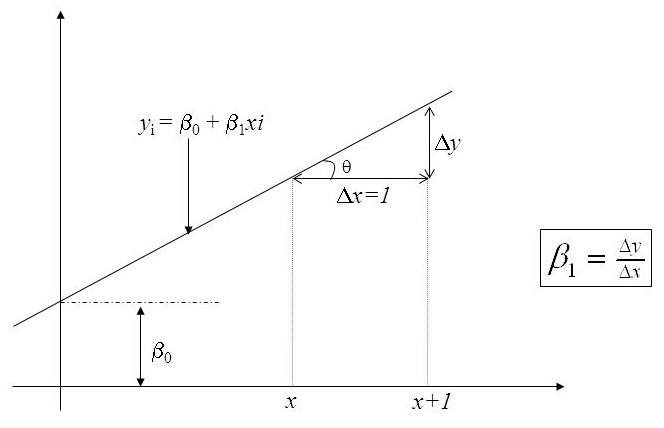
\includegraphics[scale=0.5]{Figuras/Interpretacao2}
    %\caption{Legenda}
    %\label{figRotulo}
\end{figure}
\end{block}
\end{frame}
% 
\begin{frame}{}
\frametitle{ }
\begin{block}{}
\justifying
\begin{figure}[H]
    \centering
    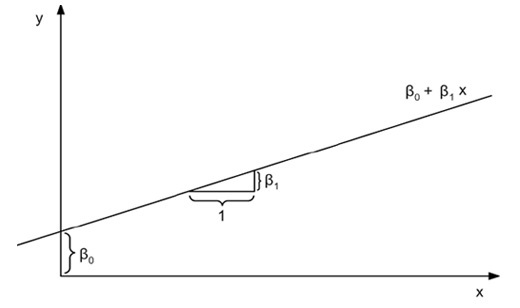
\includegraphics[scale=0.5]{Figuras/Interpretacao1}
    %\caption{Legenda}
    %\label{figRotulo}
\end{figure}
\end{block}
\end{frame}

\begin{frame}{}
\frametitle{ }
\begin{block}{}
\justifying
\begin{figure}[H]
    \centering
    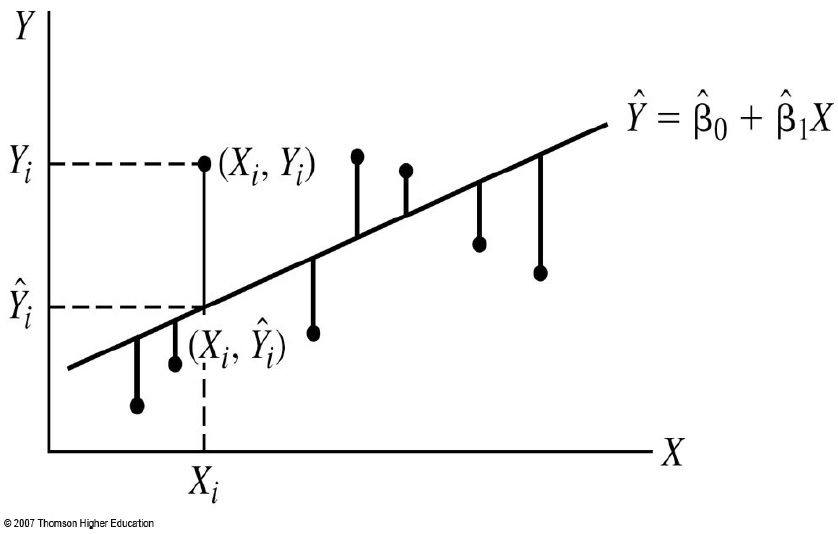
\includegraphics[scale=0.5]{Figuras/Regressao}
    %\caption{Legenda}
    %\label{figRotulo}
\end{figure}
\end{block}
\end{frame}

\begin{frame}{}
\frametitle{ }
\begin{block}{}
\justifying
\begin{figure}[H]
    \centering
    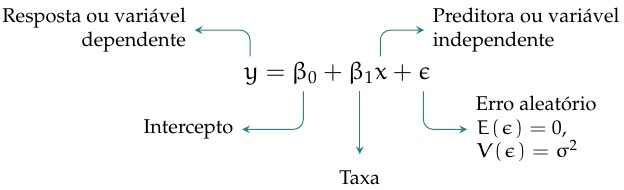
\includegraphics[scale=0.5]{Figuras/Regressao3}
    %\caption{Legenda}
    %\label{figRotulo}
\end{figure}
\end{block}
\end{frame}

\section{Pressupostos}
\begin{frame}{}
\frametitle{ }
\begin{block}{LINEARIDADE}
\justifying
(o modelo linear descreve corretamente a relação funcional entre X e Y)
Se esse pressuposto for violado a estimativa do erro aumentará, já que os valores observados não se aproximarão dos valores preditos (local onde passará a reta). Pressuposto fundamental já que essa regressão é um modelo linear.
\end{block}
\end{frame}

\begin{frame}{}
\frametitle{ }
\begin{block}{NORMALIDADE}
\justifying
Normalidade dos resíduos é esperada para que não existam tendências e que a estatística F funcione de forma correta.
\end{block}
\end{frame}

\begin{frame}{}
\frametitle{ }
\begin{block}{VARIÂNCIAS HOMOGÊNEAS}
\justifying
As variâncias dentro de cada grupo é igual (ou pelo menos aproximadamente) àquela dentro de todos os grupos. Desta forma, cada tratamento contribui de forma igual para a soma dos quadrados.
\end{block}
\end{frame}

\begin{frame}{}
\frametitle{ }
\begin{block}{}
\justifying
Se os pressupostos forem atendidos fica mais fácil afirmar que os resultados da análise são devido aos efeitos testados. Além disso, a confiabilidade do teste aumenta, já que se terá certeza que não há tendências nos resultados.
\end{block}
\end{frame}

\begin{frame}[fragile]{}
\frametitle{ }
\begin{block}{}
\justifying
Iniciemos com um exemplo. Um investigador deseja estudar a possível relação entre o salário (em mil reais) e o tempo de experiência (em anos completos) no cargo de gerente de agências bancárias de uma grande empresa. Os dados coletados são lidos no R:
\end{block}
\begin{block}{}
%\begin{Schunk}
%\begin{Sinput}
\begin{verbatim}
dados <- read.table("Exp_Salario.txt", 
                     sep = "", dec = ".", header = TRUE)
names(dados) <- c("X","Y")    
\end{verbatim}
%\end{Sinput}
%\end{Schunk}
\end{block}\pause
\begin{block}{}
são considerados 27 pares de observações correspondentes à variável resposta Salário e à variável explicativa Experiência, para cada um dos gerentes da empresa.
\end{block}
\end{frame}

\begin{frame}[fragile]{}
\frametitle{ }
\begin{block}{}
\begin{center}

%\begin{Schunk}
%\begin{Sinput}
\begin{verbatim}
plot(X,Y,xlab="Experiencia (Anos)",ylab="Salário (R$)",
      pch=16)
lines(X, fitted(lm(Y ~ X)), col="blue")    
\end{verbatim}
%\end{Sinput}
%\end{Schunk}
\end{center}
\end{block}
\vspace{-1.3cm}
\begin{center}
\setkeys{Gin}{width=0.5\linewidth}
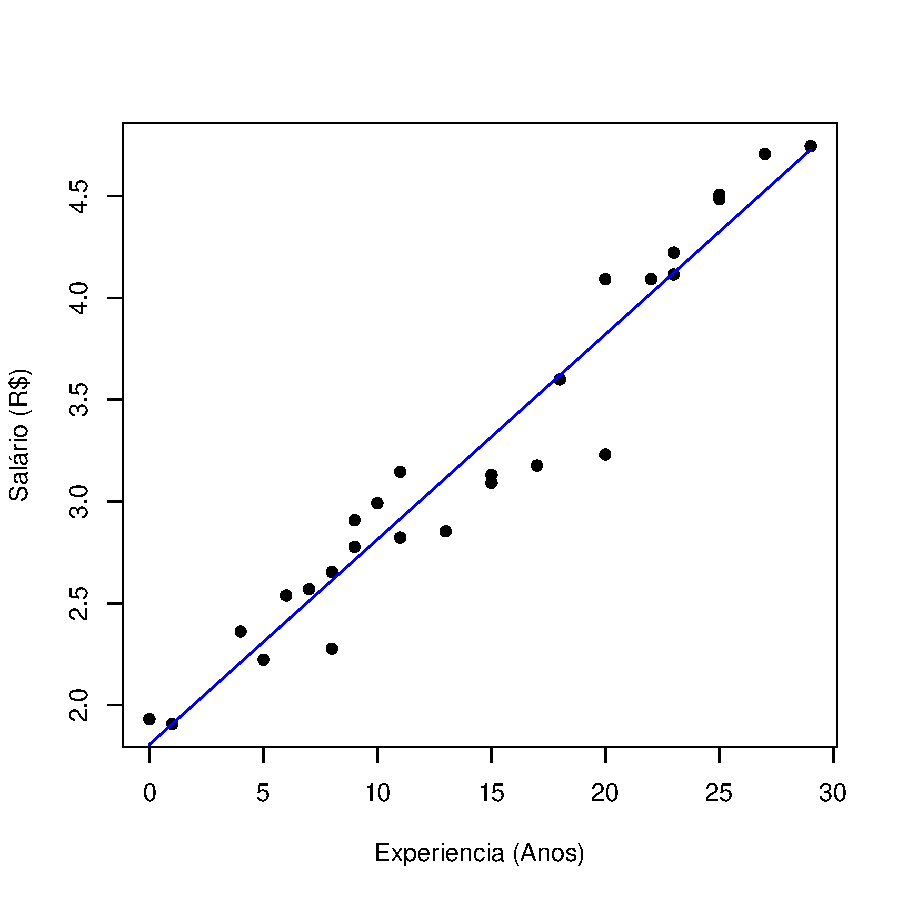
\includegraphics{Aula4Regressao/Figuras/Aula4-014}
\end{center}
\end{frame}

\begin{frame}[fragile]{}
\frametitle{ }
\begin{block}{}
%\begin{Schunk}
%\begin{Sinput}
\begin{verbatim}
cor(X,Y)    
\end{verbatim}
%\end{Sinput}
%\begin{Soutput}
\begin{verbatim}
[1] 0.9704137    
\end{verbatim}
%\end{Soutput}
%\end{Schunk}

Observe que o R retornou o valor $0.9704137$ o que evidencia uma forte relação linear entre as variáveis em estudo. Para avaliar se esse resultado é significativo, pode-se realizar um Teste de Hipóteses para o Coeficiente de Correlação.

%\begin{Schunk}
%\begin{Sinput}
\begin{verbatim}
cor.test(X,Y)    
\end{verbatim}
%\end{Sinput}
%\begin{Soutput}
\begin{verbatim}
Pearson's product-moment correlation
t = 20.096, df = 25, p-value < 2.2e-16
alternative hypothesis: true correlation is not equal to 0
95 percent confidence interval:
 0.9353175 0.9865989
\end{verbatim}
%\end{Soutput}
%\end{Schunk}
\end{block}
\end{frame}

\begin{frame}[fragile]{}
\frametitle{}
\begin{block}{}
\justifying
Para avaliar as suposições de que os erros possuem variância constante e são não correlacionados entre si, construa os gráficos de ``Resíduos versus Valores Ajustados da Variável Resposta'' e ``Resíduos versus Valores da Variável Explicativa''.
\end{block}
\end{frame}

\begin{frame}[fragile]{}
\frametitle{ }
\begin{block}{}
\justifying

%\begin{Schunk}
%\begin{Sinput}
\begin{verbatim}
m0 <- lm(Y~X)
plot(fitted(m0),residuals(m0),xlab="Valores Ajustados",
      ylab="Resíduos")
abline(h=0)
plot(X,residuals(m0),xlab="Experiência",ylab="Resíduos")
abline(h=0)
par(mfrow=c(1,2))    
\end{verbatim}
%\end{Sinput}
%\end{Schunk}
\end{block}

\end{frame}

\begin{frame}[fragile]{}
\frametitle{ }
\vspace{-0.5cm}

\begin{center}
\setkeys{Gin}{width=0.6\linewidth}
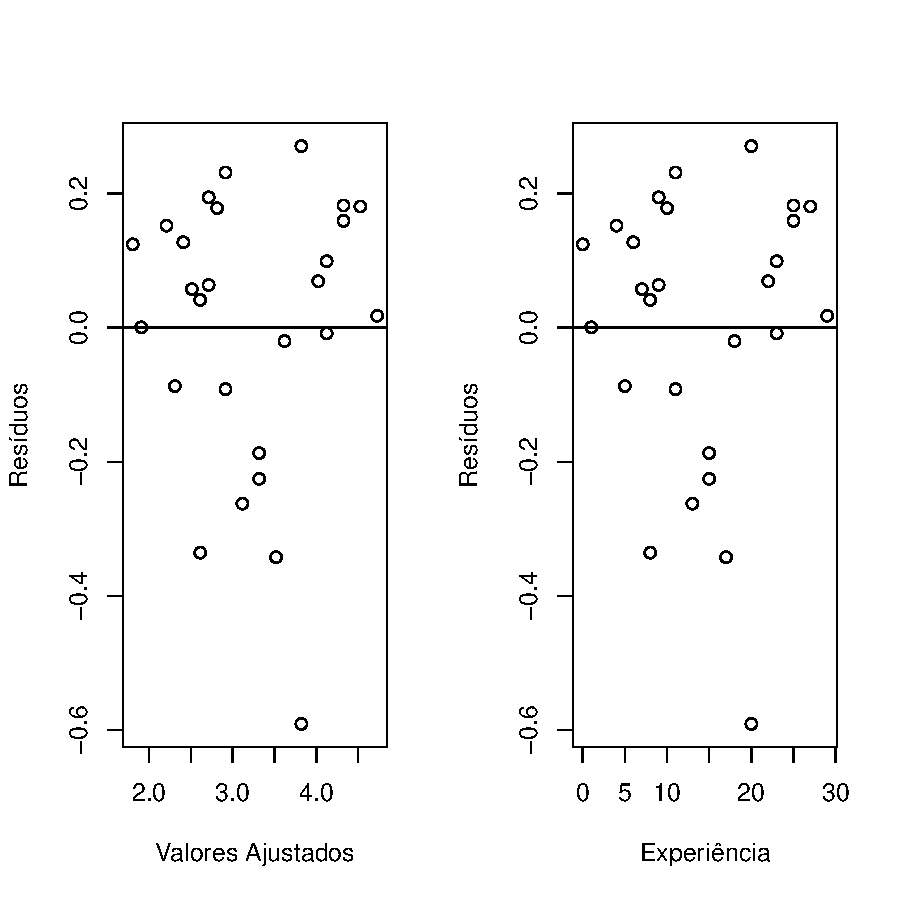
\includegraphics{Aula4Regressao/Figuras/Aula4-020}
\end{center}
\vspace{-0.5cm}
\begin{block}{}
observa-se a violação da suposição de homocedasticidade dos erros.
\end{block}
\end{frame}

\begin{frame}[fragile]{}
\frametitle{ }
\begin{block}{}
\justifying
observa-se ainda a violação da suposição de que os erros aleatórios têm distribuição
Normal. Via gráfico qqplot abaixo:
%\begin{Schunk}
%\begin{Sinput}
\begin{verbatim}
qqnorm(residuals(m0), ylab="Resíduos",
       xlab="Quantis teóricos",main="")
qqline(residuals(m0))    
\end{verbatim}
%\end{Sinput}
%\end{Schunk}
\end{block}

\vspace{-1cm}
\begin{center}
\setkeys{Gin}{width=0.4\linewidth}
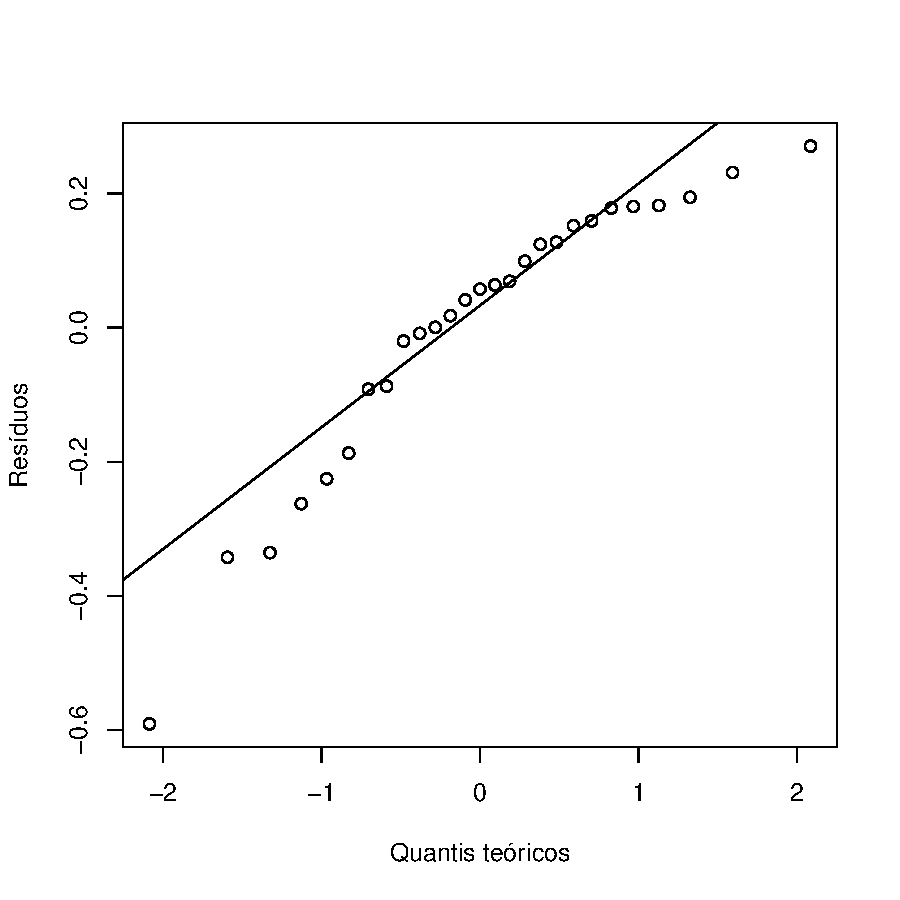
\includegraphics{Aula4Regressao/Figuras/Aula4-022}
\end{center}

\end{frame}

\begin{frame}[fragile]{}
\frametitle{ }
\begin{block}{}
%\begin{Schunk}
%\begin{Sinput}
\begin{verbatim}
shapiro.test(residuals(m0))    
\end{verbatim}
%\end{Sinput}
%\begin{Soutput}
\begin{verbatim}
	Shapiro-Wilk normality test

data:  residuals(m0)
W = 0.9012, p-value = 0.01425    
\end{verbatim}
%\end{Soutput}
%\end{Schunk}
\end{block}
\end{frame}

\begin{frame}[fragile]{}
\frametitle{ }
\begin{block}{Calculamos $\sqrt{Y}$ e reaplicamos o modelo linear}
\vspace{-0.5cm}
\end{block}
\begin{center}
\setkeys{Gin}{width=0.5\linewidth}
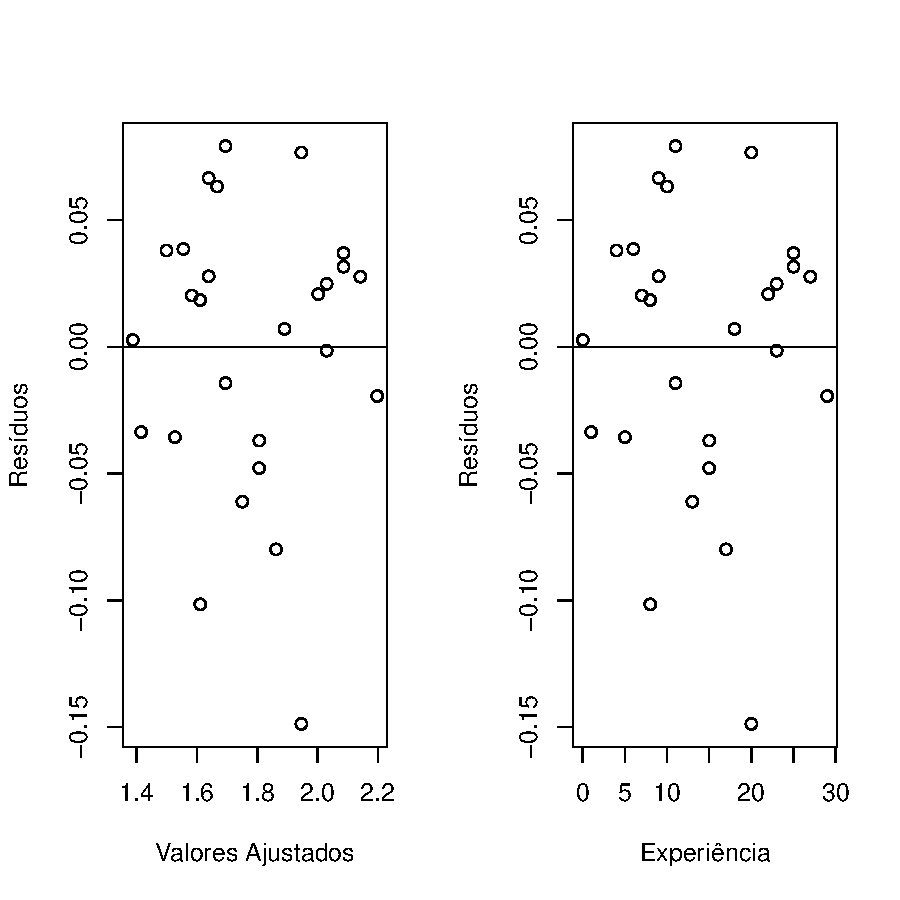
\includegraphics{Aula4Regressao/Figuras/Aula4-024}
\end{center}
\end{frame}
% 
\begin{frame}[fragile]{}
\frametitle{ }
\begin{block}{Calculamos $\sqrt{Y}$ e reaplicamos o modelo linear}

observa-se a não violação da suposição de homocedasticidade dos erros.

\begin{center}
%\setkeys{Gin}{width=0.5\linewidth}
%\begin{Schunk}
%\begin{Soutput}
\begin{verbatim}
	Shapiro-Wilk normality test

data:  residuals(m1)
W = 0.94139, p-value = 0.1319    
\end{verbatim}
%\end{Soutput}
%\end{Schunk}
\end{center}
\end{block}
\end{frame}
% 
% 
\begin{frame}[fragile]{}
\frametitle{ }
\begin{block}{}
\justifying


%\begin{Schunk}
%\begin{Sinput}
\begin{verbatim}
qqnorm(residuals(m1), ylab="Resíduos",
        xlab="Quantis teóricos",main="")
qqline(residuals(m1))    
\end{verbatim}
%\end{Sinput}
%\end{Schunk}
\end{block}

%\begin{block}{}
\vspace{-1cm}
\begin{center}
\setkeys{Gin}{width=0.5\linewidth}
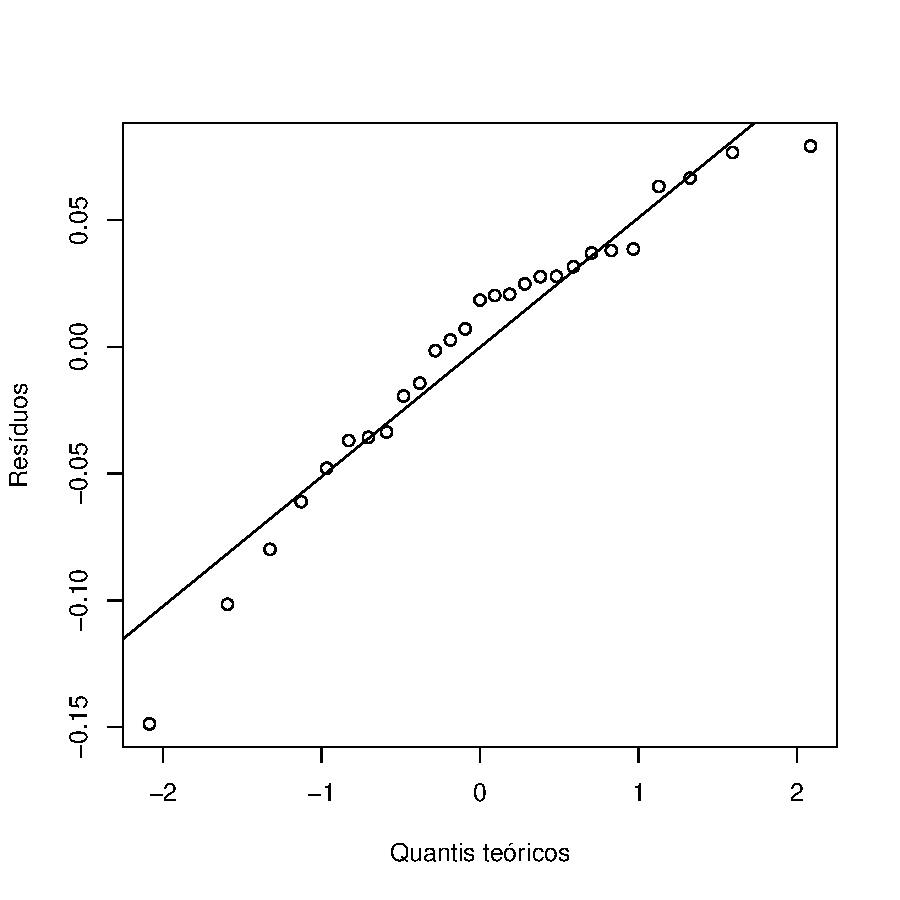
\includegraphics{Aula4Regressao/Figuras/Aula4-028}
\end{center}
%\end{block}
\end{frame}

\begin{frame}[fragile]{}
\frametitle{ }
\begin{block}{Calculamos $\sqrt{Y}$ e reaplicamos o modelo linear}
%\begin{Schunk}
%\begin{Sinput}
\begin{verbatim}
dados <- read.table("Exp_Salario.txt",
                     sep = "", dec = ".", header = TRUE)
names(dados) <- c("X","Y")
attach(dados)
m1 <- lm(sqrt(Y)~X)
m1    
\end{verbatim}
%\end{Sinput}
%\begin{Soutput}
\begin{verbatim}
Call:
lm(formula = sqrt(Y) ~ X)

Coefficients:
(Intercept)            X  
    1.38680      0.02797     
\end{verbatim} 
%\end{Soutput}
%\end{Schunk}
\end{block}
\end{frame}

\begin{frame}[fragile]{}
\frametitle{ }
\begin{block}{Calculamos $\sqrt{Y}$ e reaplicamos o modelo linear}

%\begin{Schunk}
%\begin{Sinput}
\begin{verbatim}
summary(m1)    
\end{verbatim}
%\end{Sinput}
%\begin{Soutput}
\begin{verbatim}
lm(formula = sqrt(Y) ~ X)

Coefficients:
            Estimate Std. Error t value Pr(>|t|)    
(Intercept)  1.38680    0.02165   64.06   <2e-16 ***
X            0.02797    0.00133   21.03   <2e-16 ***
---
Signif. codes:  0 '***' 0.001 '**' 0.01 '*' 0.05 '.' 
Residual standard error: 0.05606 on 25 degrees of freedom
Multiple R-squared:  0.9465,	Adjusted R-squared:  0.9444 
F-statistic: 442.3 on 1 and 25 DF,  p-value: < 2.2e-16 
\end{verbatim}
%\end{Soutput}
%\end{Schunk}

\end{block}
\end{frame}

\end{document}
